%%%%%%%%%%%%%%%%%%%%%%%%%%%%%%%%%%%%%%%%%
% a0poster Portrait Poster
% LaTeX Template
% Version 1.0 (22/06/13)
%
% The a0poster class was created by:
% Gerlinde Kettl and Matthias Weiser (tex@kettl.de)
% 
% This template has been downloaded from:
% http://www.LaTeXTemplates.com
%
% License:
% CC BY-NC-SA 3.0 (http://creativecommons.org/licenses/by-nc-sa/3.0/)
%
%%%%%%%%%%%%%%%%%%%%%%%%%%%%%%%%%%%%%%%%%
% Perrinet18gdr
\newcommand{\Author}{Laurent U.~Perrinet}%
\newcommand{\Address}{Institut de Neurosciences de la Timone\\CNRS / Aix-Marseille Universit\'e - Marseille, France}%
\newcommand{\Website}{http://invibe.net/LaurentPerrinet}%
\newcommand{\Title}{A low-cost, accessible eye tracking framework}%
\newcommand{\Email}{laurent.perrinet@univ-amu.fr}%

\documentclass[a0,portrait]{a0poster}

\usepackage{multicol} % This is so we can have multiple columns of text side-by-side
\columnsep=100pt % This is the amount of white space between the columns in the poster
\columnseprule=0pt % This is the thickness of the black line between the columns in the poster
\usepackage{url}

\usepackage[svgnames]{xcolor} % Specify colors by their 'svgnames', for a full list of all colors available see here: http://www.latextemplates.com/svgnames-colors

\usepackage{times} % Use the times font
%\usepackage{palatino} % Uncomment to use the Palatino font

\usepackage{graphicx} % Required for including images
\graphicspath{{figures/}} % Location of the graphics files
\usepackage{booktabs} % Top and bottom rules for table
\usepackage[font=small,labelfont=bf]{caption} % Required for specifying captions to tables and figures
\usepackage{amsfonts, amsmath, amsthm, amssymb} % For math fonts, symbols and environments
\usepackage{wrapfig} % Allows wrapping text around tables and figures

\usepackage{natbib}
\begin{document}

%----------------------------------------------------------------------------------------
%	POSTER HEADER 
%----------------------------------------------------------------------------------------

% The header is divided into two boxes:
% The first is 75% wide and houses the title, subtitle, names, university/organization and contact information
% The second is 25% wide and houses a logo for your university/organization or a photo of you
% The widths of these boxes can be easily edited to accommodate your content as you see fit

\begin{minipage}[b]{0.75\linewidth}
%\VeryHuge
\Huge \color{Navy} \textbf{\Title} \color{Black}\\[0.9cm] % Title
%\Huge\textit{Country Update}\\[2.4cm] % Subtitle
\huge \textbf{\Author} \\[0.9cm] % Author(s)
\huge \Address\\[0.4cm] % University/organization
\Large \texttt{\Email} \\
\end{minipage}
%
\begin{minipage}[b]{0.25\linewidth}

\includegraphics[width=13cm]{Logo_int.png}\ 

\includegraphics[width=10.5cm]{Logo_amu.png}\\
\end{minipage}

\vspace{2cm} 
%----------------------------------------------------------------------------------------

\begin{multicols}{3} % This is how many columns your poster will be broken into, a portrait poster is generally split into 2 columns

%----------------------------------------------------------------------------------------
%	ABSTRACT
%----------------------------------------------------------------------------------------

\color{Navy} % Navy color for the abstract

\begin{abstract}
Recording eye movements is a technique that attracts an increasing number of scientists, but also in the general public. Indeed, this allows to quantitatively measure a number of useful dimensions of perception and behavior in general. However, most existing trackers rely on expensive or technically complex solutions. Here, we propose a simple framework to record eye movements using any camera, such as a webcam. As a proof of concept, the recorded image is processed in real-time to detect from a simple sub-set of eye movements : left, center, right or blink. The processing is based on two stages. First, we use a pre-trained computer vision algorithm to extract the image of the face. Second, we used a classical deep-learning architecture to learn to classify these sub-images. This network is a $3$ layered convolutional neural network, for which we optimized performance as measured by the accuracy with cross-validation on a wide range of the network's hyper-parameters. Over a dataset of more than $1000$ images, this network achieves an average accuracy of approximately $97$\%. We also provide with an integration with the psychopy library which shows that frames can be processed on a standard laptop at a rate of approximately~$25$~Hz.
\end{abstract}
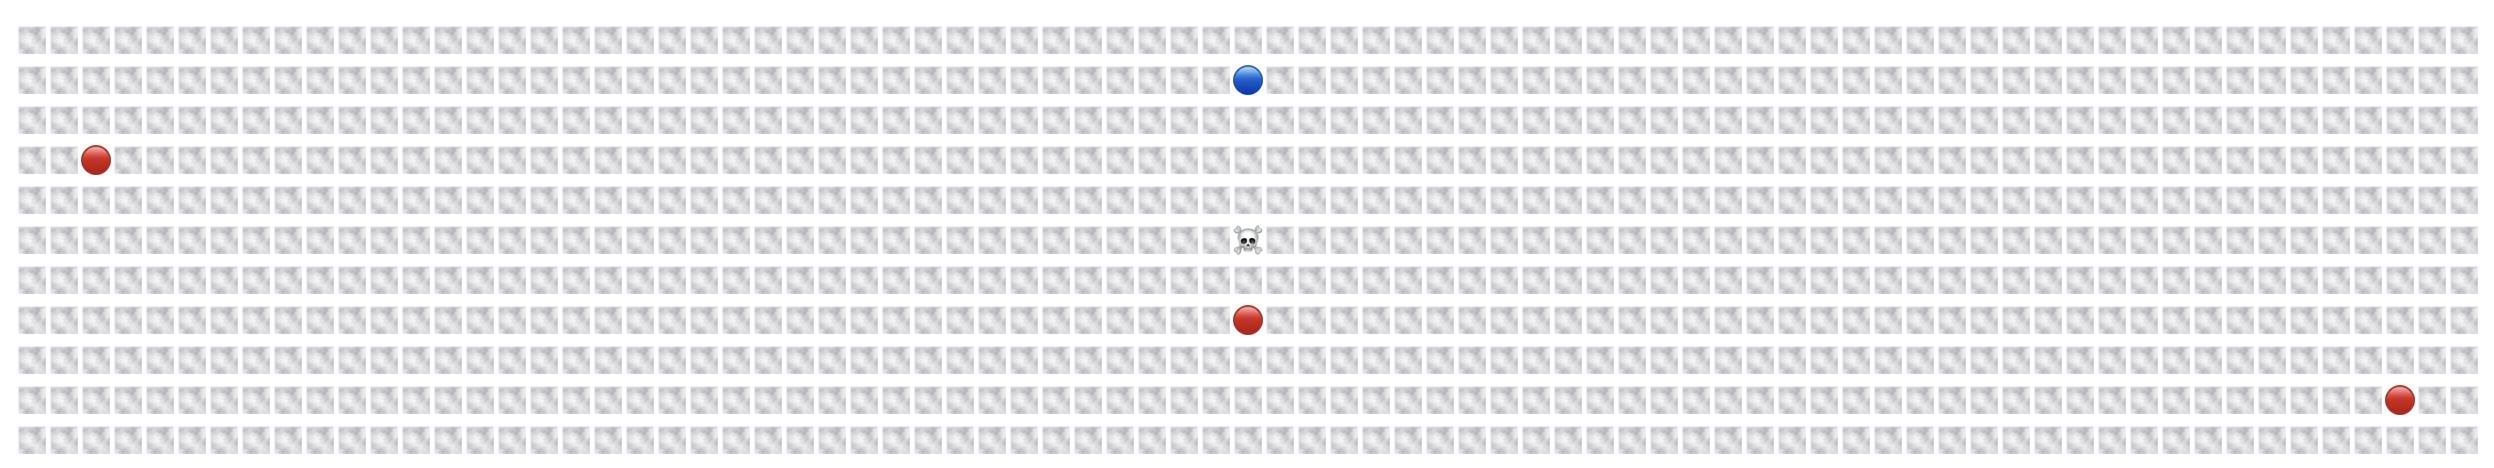
\includegraphics[width=1.\linewidth, height=.2\linewidth]{stimuli.png}

%----------------------------------------------------------------------------------------
%	INTRODUCTION
%----------------------------------------------------------------------------------------
\color{Black} % SaddleBrown color for the introduction
%\section*{LeCheapEyeTracker: low cost, low precision, high accuracy}
\section*{Why another eye tracker?}
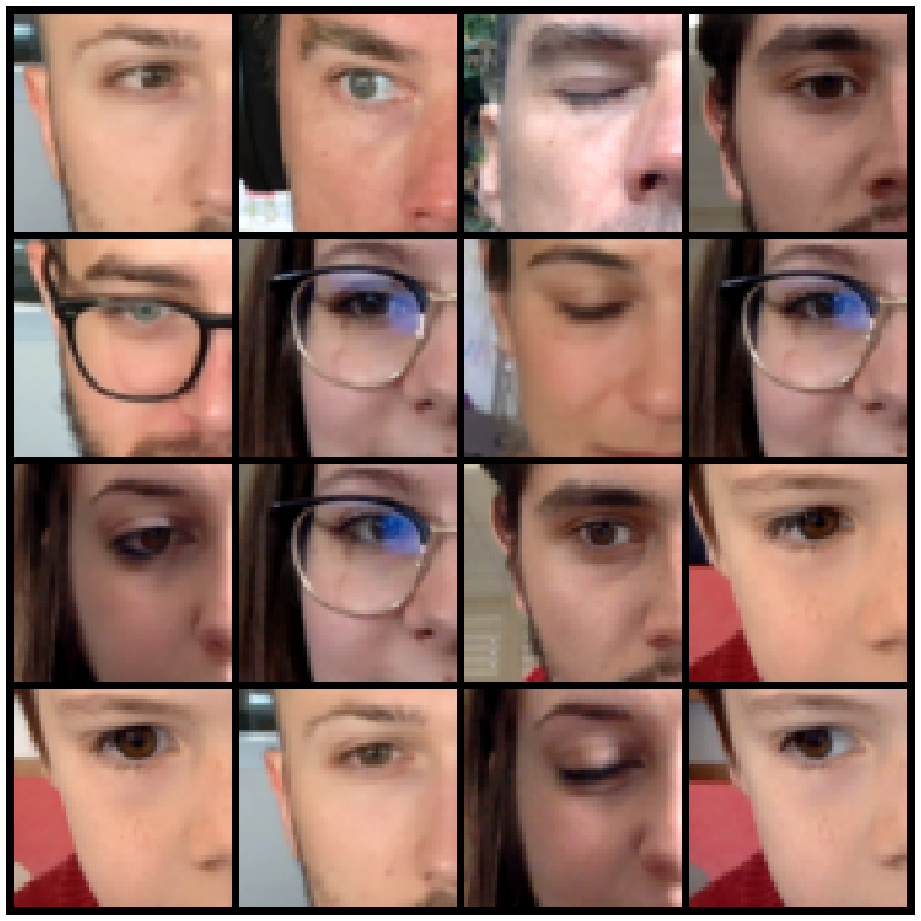
\includegraphics[width=1.\linewidth]{dataset.pdf}
\captionof{figure}{\color{DarkSlateGray} We investigated the performance of this novel, low-cost, low-precision eye tracker. First, we capture full scale images of the scene using the openCV library. , we extract the bounding box around the face in that scene using the DLib library~\citep{dlib09}. In the learning phase, we order the extracted images using 4 labels: `center', `left', `right' and `blink'. These labels are then used to supervise the learning of the association between the input image of the extracted image and the output label.}


\includegraphics[width=1.\linewidth]{accuracy.pdf}
\captionof{figure}{\color{DarkSlateGray} The learning was performed using the pytorch library~\citep{paszke2017automatic} over $20$ epochs. Accuracy was tested on 20 cross-validations.  Over a dataset of more than $1000$ images, this network achieves an average accuracy of approximately $97$\%.
}
%----------------------------------------------------------------------------------------


\end{multicols}

\vspace{4cm} 

\color{Black} % DarkSlateGray 
\begin{minipage}{0.67\linewidth}
\section*{Recognition model: a classical convolutional neural network}
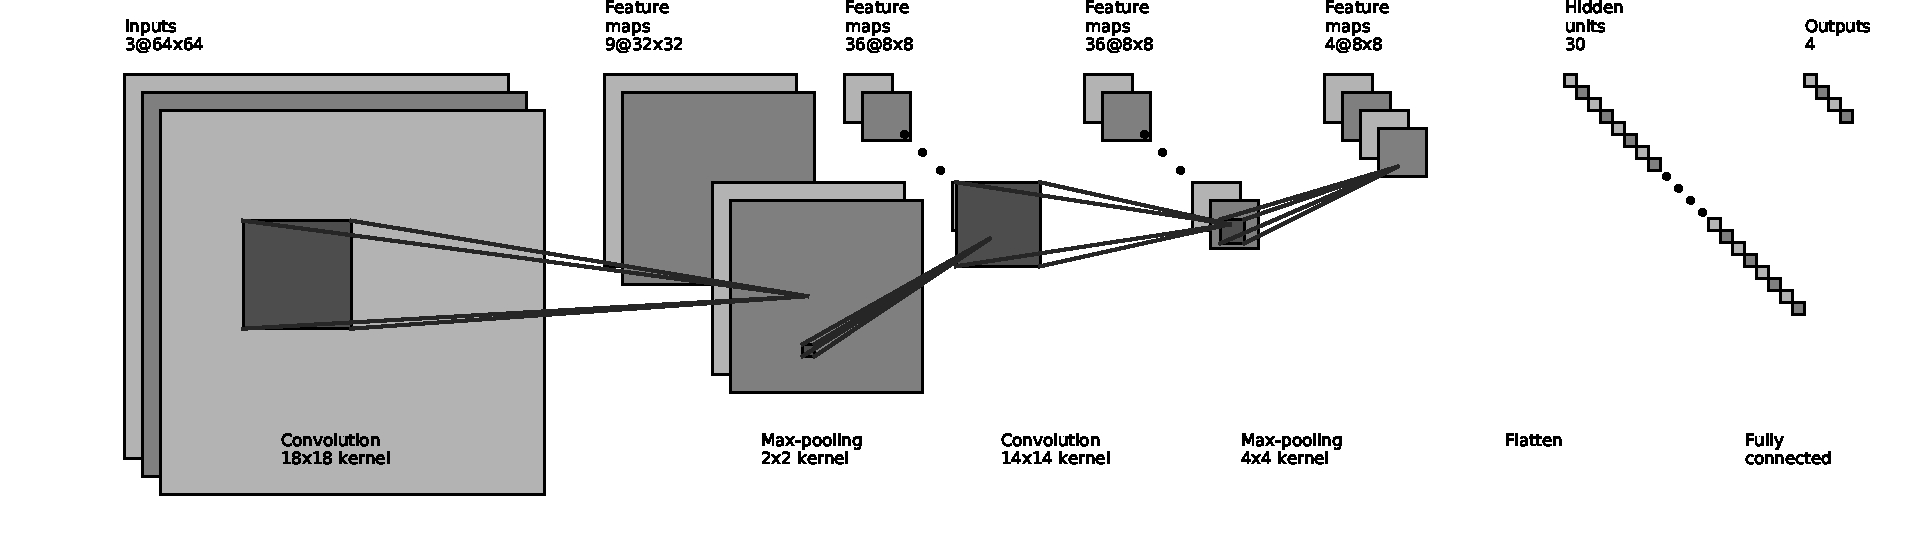
\includegraphics[width=1\linewidth]{CNN.pdf}
%----------------------------------------------------------------------------------------
\end{minipage}
\begin{minipage}{0.3\linewidth}
\captionof{figure}{\color{DarkSlateGray} The architecture of the original convolutional neural network, as introduced by~\citep{lecun1989backpropagation,lecun1998gradient}, alternates between convolutional layers including rectifying non-linearities and max-pooling layers layers. The feature maps of the final subsampling (striding) layer are then fed into two layers of fully connected neurons. The output layer uses softmax activation functions to generate a decision. Our model was trained on more than 1000 images taken from a standard desktop / laptop webcam. The implementation relies on the pytporch library~\citep{paszke2017automatic}, such that learning is performed in approximately $700$ seconds (GPU standalone server with a GeForce GTX 1060 Nvidia card) and that the forward pass takes approximately $2$ milliseconds. }
\end{minipage}\hfil


\vspace{3cm} 

\section*{Quantitative performance over the set of free parameters}
\vspace{2cm} 

\begin{center}
\begin{minipage}{.9334\linewidth}
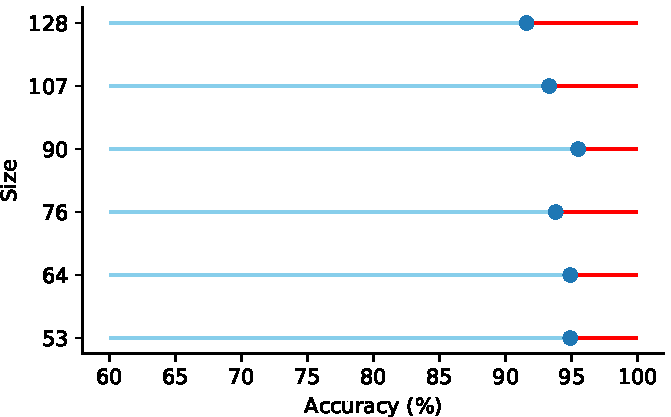
\includegraphics[width=.13333\linewidth]{accuracy_size.pdf} 
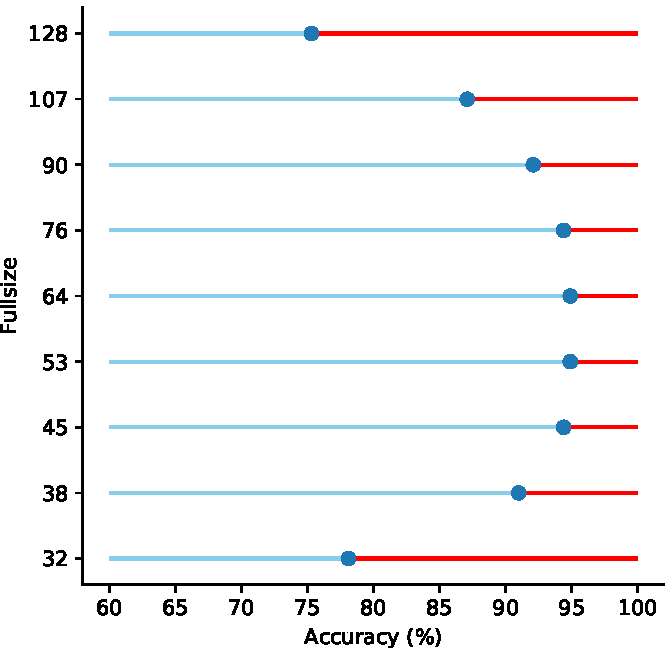
\includegraphics[width=.13333\linewidth]{accuracy_fullsize.pdf} 
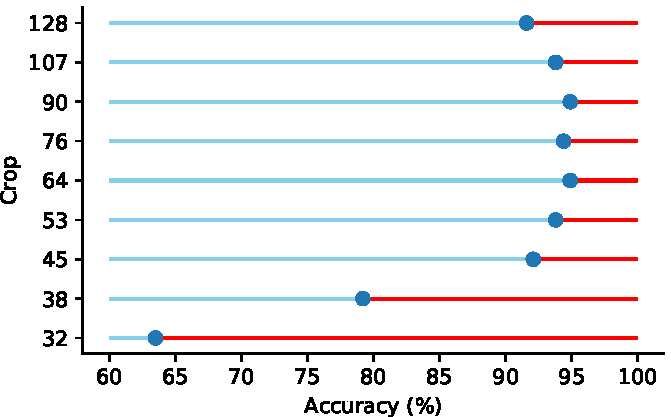
\includegraphics[width=.13333\linewidth]{accuracy_crop.pdf} 
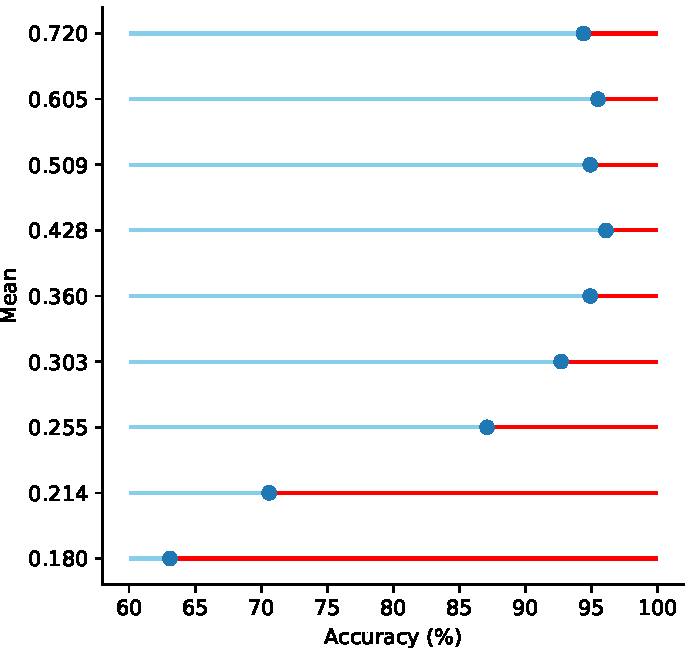
\includegraphics[width=.13333\linewidth]{accuracy_mean.pdf} 
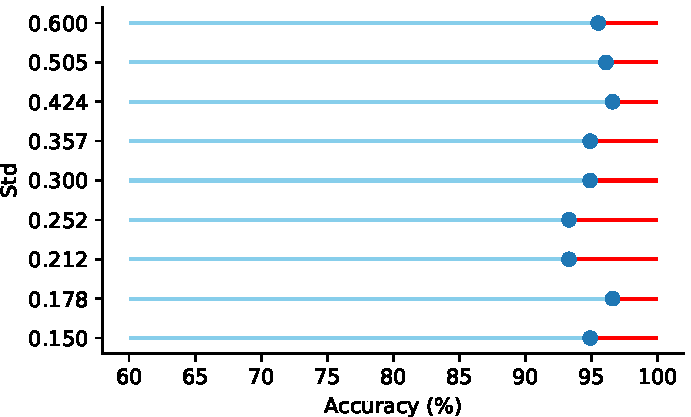
\includegraphics[width=.13333\linewidth]{accuracy_std.pdf} 
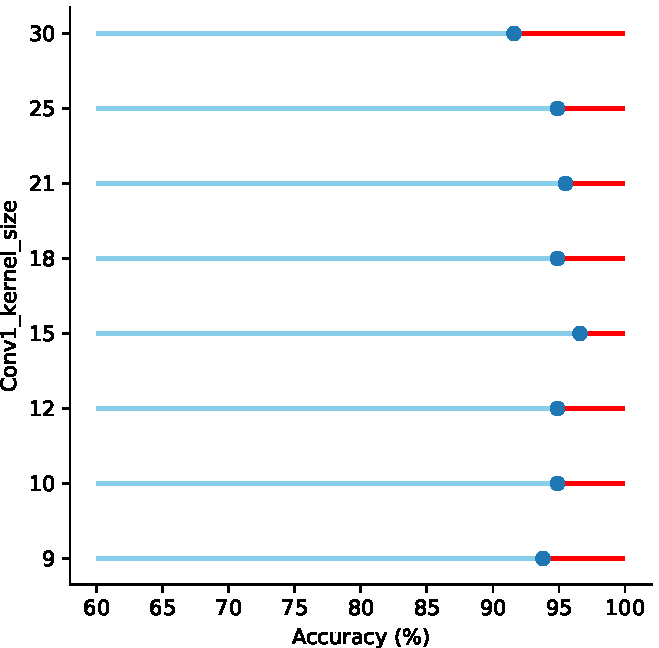
\includegraphics[width=.13333\linewidth]{accuracy_conv1_kernel_size.pdf} 
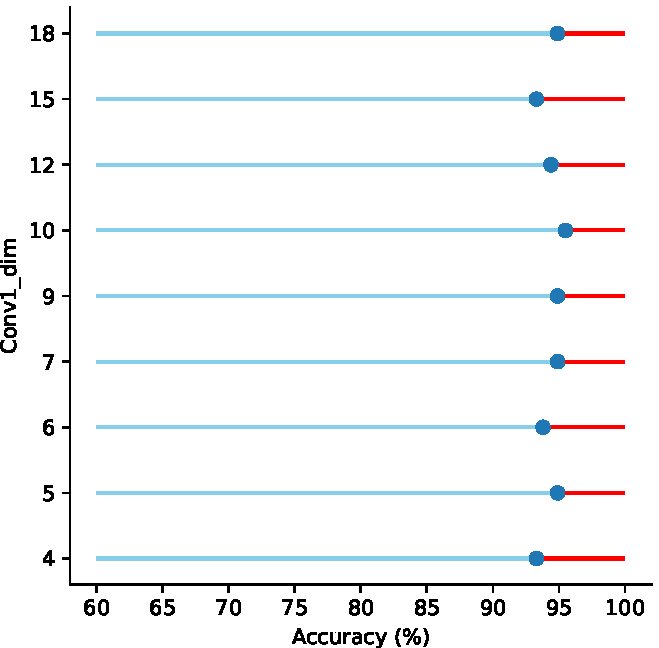
\includegraphics[width=.13333\linewidth]{accuracy_conv1_dim.pdf} \\
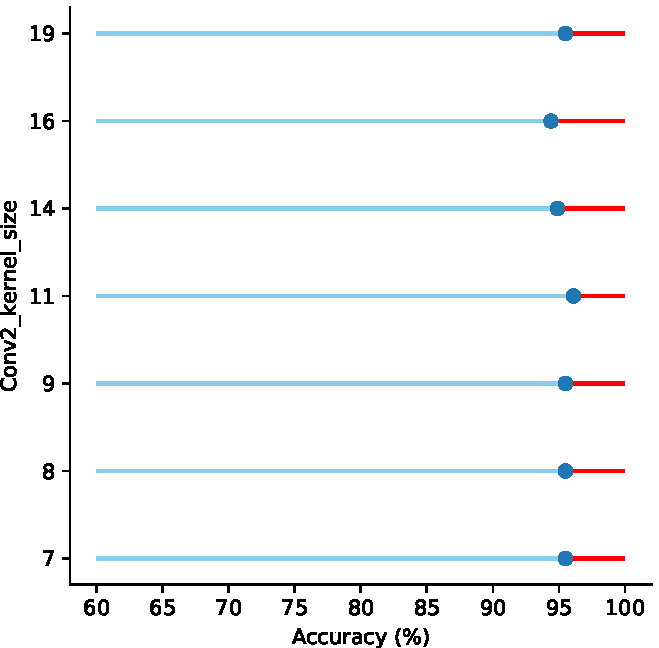
\includegraphics[width=.13333\linewidth]{accuracy_conv2_kernel_size.pdf} 
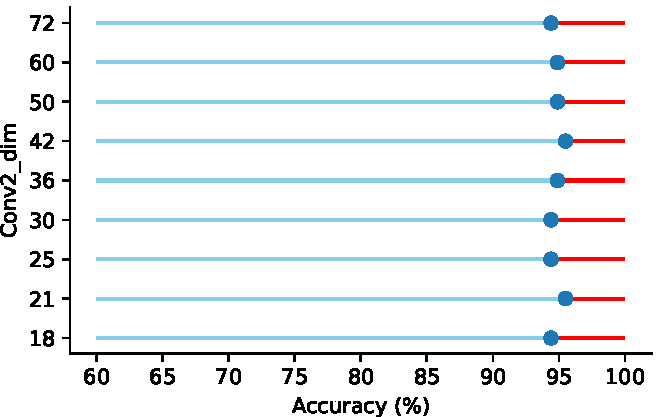
\includegraphics[width=.13333\linewidth]{accuracy_conv2_dim.pdf} 
%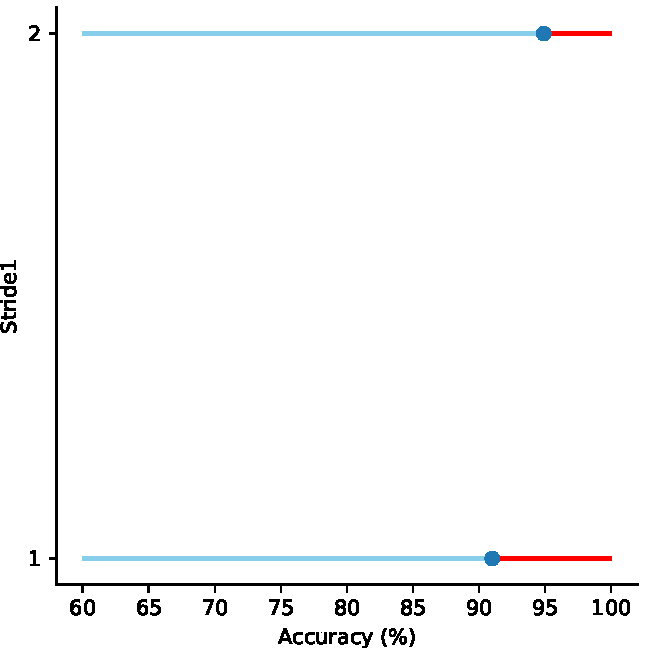
\includegraphics[width=.13333\linewidth]{accuracy_stride1.pdf} 
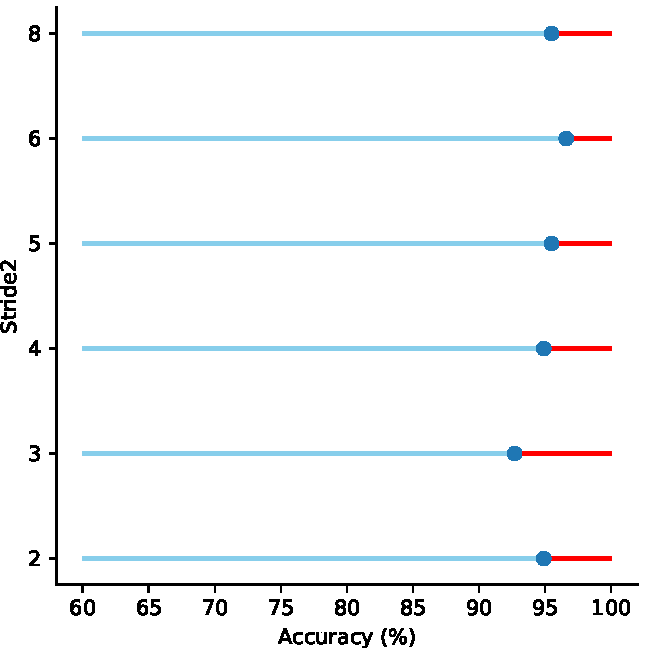
\includegraphics[width=.13333\linewidth]{accuracy_stride2.pdf} 
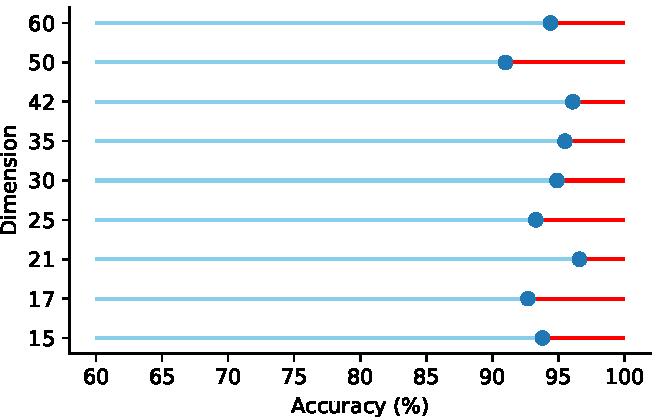
\includegraphics[width=.13333\linewidth]{accuracy_dimension.pdf} 
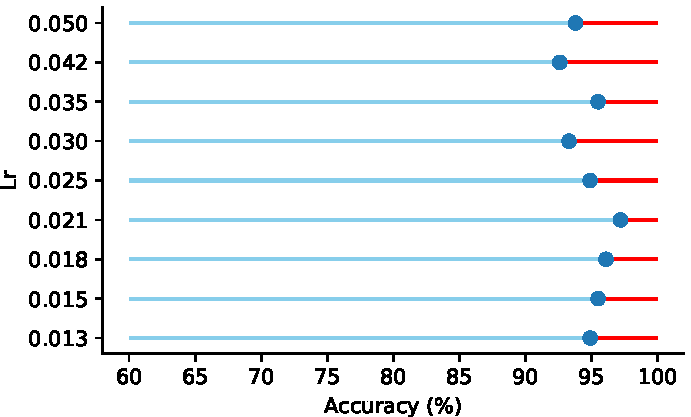
\includegraphics[width=.13333\linewidth]{accuracy_lr.pdf} 
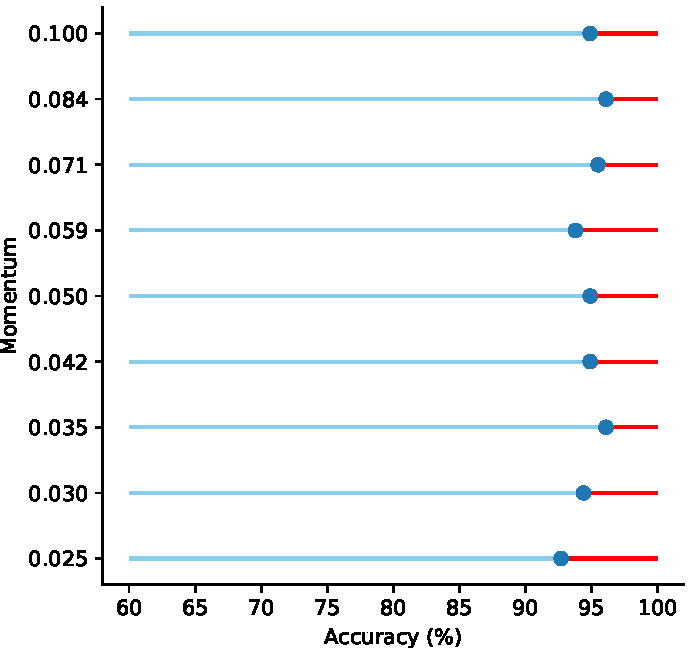
\includegraphics[width=.13333\linewidth]{accuracy_momentum.pdf} 
%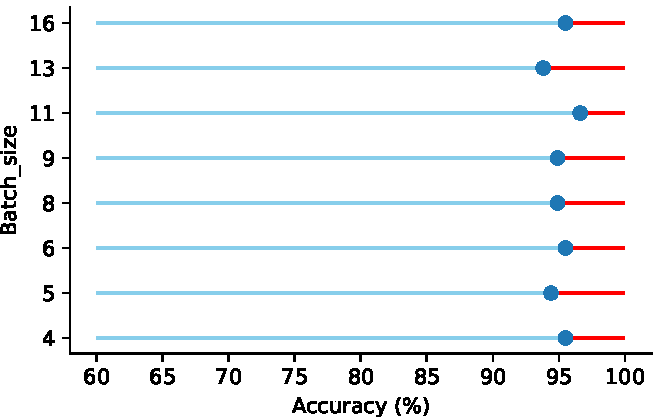
\includegraphics[width=.13333\linewidth]{accuracy_batch_size.pdf} 
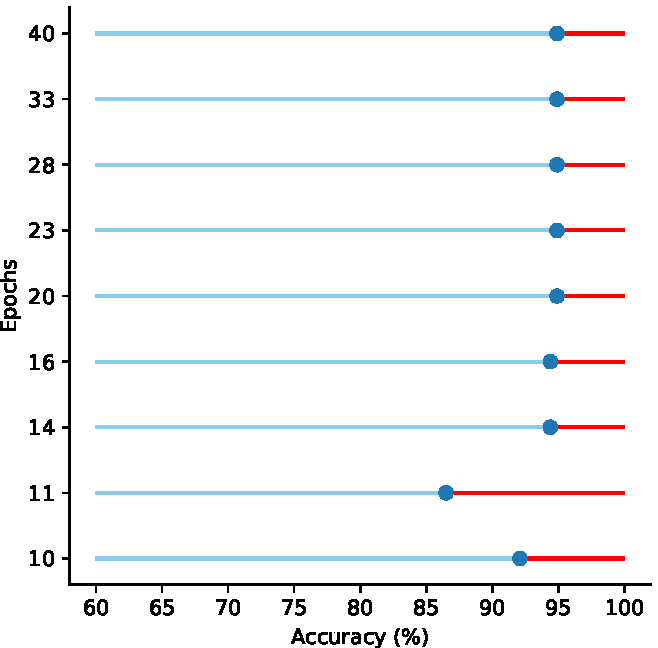
\includegraphics[width=.13333\linewidth]{accuracy_epochs.pdf}
\end{minipage}
\end{center}

\vspace{2cm} 

\begin{multicols}{3} % This is how many columns your 
\color{Navy} % Navy color for the abstract

\section*{Conclusions}
We have shown here that a simple architecture could allow for a low-cost, accessible eye tracking framework with a high accuracy ($>97\%$). One drawback of this architecture is its low-precision (4 bit output). This precision can certainly be improved by using more complex network architectures such as state-of-the art deep learning architectures. We envision that such a framework could be used in a wide range of human machine interfaces (laptops, tablets, smartphones). Also, we have exploited each frame independently and we expect to be able to achieve a higher temporal accuracy when handling the input sequence dynamically by extendng the input to several frames.

\color{Black} % Set the color back to DarkSlateGray for the rest of the content

\section*{Additional resources}

\begin{minipage}{0.3\linewidth}

\includegraphics[width=1.\linewidth]{GitQR.png}
\end{minipage}\hfil
\begin{minipage}{0.67\linewidth}
The model and data are open-source. You can either flash the code or go to \url{https://invibe.net/LaurentPerrinet/Publications/Perrinet18gdr}
\end{minipage}

\bibliographystyle{plain} % Plain referencing style
\bibliography{Perrinet18gdr} % Use the example bibliography file sample.bib
%--------------------------------------------------------------------------------
\end{multicols}
\end{document}